\section{Lecture 35}
\subsection{Lecture Notes - Course Review II}
\subsubsection{Examples of Canonical Transformations}
Only transformations in which new coordinates obey Hamilton's equations of motion are canonical. Suppose we have our generalized position $q$ that maps to a new variable $Q = p$ and our generalized momentum $p$ that maps to a new variable $P = -q$. The original coordinates satisfy Hamilton's equations, so:
\[\dot{q} = \dpd{\HH}{p}, \quad \dot{p} = -\dpd{\HH}{q}\]
We therefore have that:
\[\dot{Q} = \dot{p} = -\dpd{\HH}{q} = -\dpd{\HH}{(-P)} = \dpd{\HH}{P}\]
So the first equation of motion is satisfied. Playing the same game with $\dot{P}$, we have:
\[\dot{P} = -\dot{q} = -\dpd{\HH}{p} = -\dpd{\HH}{Q}\]
So this also works out. Checking the (fundamental) Poisson brackets, we have that:
\[[Q, Q] = [p, p] = 0\]
\[[P, P] = [-q, -q] = [q, q] = 0\]
\[[Q, P] = [p, -q] = -[p, q] = -(-[q, p]) = [q, p] = 1\]
So we have checked that this is a canonical transformation in a completely equivalent way. Recall that we can come up with generating functions $F$ which link the old and new variables. One example (in the HW) was:
\[F_1(q, Q) = qe^Q\]
Now we can calculate the momenta:
\[p_i = \dpd{F_1}{q_i}, \quad P_i = -\dpd{F_i}{Q_i}\]
A second example is:
\[F_2(p, Q) = -(e^Q - 1)^2\tan p\]
Where:
\[q_i = -\dpd{F_2}{p_i}, \quad P_i = -\dpd{F_2}{Q_i}\]
The significance of all of this is that there is a subclass of transformations, where due to the Jacobian determinant being equal to 1, the metric of phase space is preserved (this relates to a fundamental symmetry). 

\subsubsection{Practice Problem}
\begin{center}
    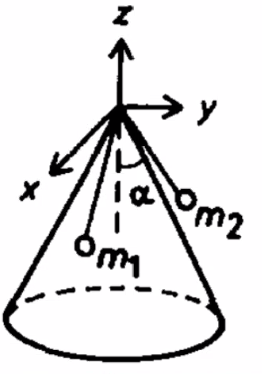
\includegraphics[scale=0.5]{Lecture-35/l35-img1.png}
\end{center}
Two equal masses are connected by a string of length $l$ that runs through the tip of a cone. One mass is free to move inside, the other moves without friction on the surface. 
\begin{enumerate}
    \item Set up suitable generalized coordinates.
    \begin{s}
    It is most natural to use spherical. For $m_1$ we use coordinates $(r, \theta, \phi)$. For $m_2$ we have coordinates $(l - r, \pi - \alpha, \beta)$. We have 6 variables, 4 independent, and two constrains. We put origin at the top of the cone. Take $r, \theta, \phi, \beta$ as our generalized coordinates.
    \end{s}
    \item Find the Lagrangian and the equations of motion. Are there cylical coordinates?
    \begin{s}
    Velocities are given by:
    \[m_1: (\dot{r}, r\dot{\theta}, r\dot{\phi}\sin\theta)\]
    \[m_2: (-\dot{r}, 0, (l-r)\dot{\beta}\sin(\pi - \alpha))\]
    \[\LL = \frac{m}{2}\left[2\dot{r}^2 + r^2\dot{\theta}^2 + r^2\dot{\phi}^2\sin^2\theta + (l-r)\dot{\beta}^2\sin^2(\pi - \alpha)\right] - mgr\cos\theta + mg(l-r)\cos\alpha\]
    To find the equations of motion, we use the Euler Lagrange equations. We notice that the Lagrangian has no dependence on $\phi$ or $\beta$ and hence these coordinates are cyclic.
    \end{s}
    \item Find the Hamiltonian.
    \begin{s}
    For the cyclic coordinates, we have:
    \[p_\phi = mr^2\dot{phi}\sin^2\theta = \text{Const.}\]
    \[p_\beta = m(l-r)^2\dot{\beta}\sin^2(\pi - \alpha) = \text{Const.}\]
    For the $r$ equations, we have:
    \[2\ddot{r} - r(\dot{\theta}^2 + \dot{\phi}^2\sin^2\theta) + (l-r)\dot{\beta}^2\sin\alpha + g(\cos\theta + \cos\alpha) = 0\]
    For the $\theta$ equation we have:
    \[r\ddot{\theta} + 2\dot{r}\dot{\theta} - r\dot{\phi}^2 = \]
    \end{s}
    \item What is the angular velocity of the particle on the outside if it moves in a circular orbit?
    \begin{s}
    We already calcualted $p_\phi$ and $p_\theta$ which were constant. Calculating the other two, we have:
    \[p_r = \dpd{\LL}{\dot{r}} = 2m\dot{r}\]
    \[p_\theta = \dpd{\LL}{\dot{\theta}} = mr^2\dot{\theta}\]
    The Hamiltonian is given by:
    \[\HH = p_r\dot{r} + p_\theta\dot{\theta} + p_\phi\dot{\phi} + p_\beta\dot{\beta} - \LL\]
    Hence:
    \[\HH = \frac{p_r^2}{2m} + \frac{p_\theta^2}{2mr^2} + \frac{p_\phi^2}{2mr\sin^2\theta} + \frac{p_\beta^2}{2m(l-r)^2\sin^2\alpha} + mgr\cos\theta - mg(L-r)\cos\alpha\]
    Here we see that the Hamiltonian is just $\HH = T + U$ as the transformation is indeed natural. Moving onto solving the question, in a circular orbit $r = \text{Const.}$, so we can therefore solve for:
    \[\dot{\beta} = \frac{p_\beta^2}{2m(l-r)^2\sin^2\alpha}\]
    \end{s}
\end{enumerate}